% =====================================================================
%  Chapter 2 — Creating and setting up your organization
%  Status: under review
% =====================================================================
\chapter{Creating and setting up your organization}
\label{ch:org-setup}

\section{Setup result}
\label{sec:setup-minute}

\textbf{Who:} the setup administrator handles this stage once. \textbf{Result:} the stage ends with a ready organization the administrator can sign in to, with its language, time zone and start of week set and saved.

If your organization already exists, do not create another copy; review its data and complete whatever is missing.

\begin{figure}[H]
\centering
\begin{tikzpicture}[node distance=0.45cm,stepBox/.append style={minimum width=5cm,text width=4.6cm,minimum height=0.7cm,font=\small\bfseries}]
  \node[stepBox]            (s1) {Create the\\organization};
  \node[stepBox,below=of s1] (s2) {Organization settings};
  \node[stepBox,below=of s2] (s3) {Check sign-in\\and settings};
  \foreach \a/\b in {s1/s2,s2/s3} \draw[flowsTo] (\a) -- (\b);
\end{tikzpicture}
\rclegend
\caption{Create the organization and check its settings}
\label{fig:setup-steps}
\shotnote{The figure summarizes the three setup stages in order: create the organization, adjust its settings, then check sign-in and settings together. Do not move on before saving the previous stage; if your organization already exists, start at the first stage not yet done.}
\end{figure}

\section{Before you start}
\label{sec:setup-before}

Prepare the organization details, contact method and administrator account listed below. You will add team records in the HR chapter.

\textbf{Subdomain:} your organization’s own part of the sign-in address; it comes at the start of the address.

\begin{rcnote}[Example: Horizon]
Horizon’s subdomain is hzn, so its sign-in address is hzn.kayanos.app.
\end{rcnote}

\begin{table}[H]
\centering
\caption{What to prepare before creating the organization}
\label{tab:setup-before}
\rcZebra
\begin{tabularx}{\linewidth}{R{4cm} R{2.4cm} Y}
\rcHeaderRow
\thh{Item} & \thh{Type} & \thh{Note}\\
Email or phone number & \req & Receives the verification code.\\
Organization name & \req & Can be written in more than one language.\\
Subdomain & \req & A unique part of the sign-in address.\\
Country and number of employees & \req & The number of employees is an estimate (a range).\\
Admin name & \req & The owner of the first account.\\
Admin password & \opt & If left empty, you receive a code to set it later.\\
Logo & \opt & An image up to 5 MB.\\
\end{tabularx}
\end{table}

\section{1. Create the organization}
\label{sec:setup-create}

From sign-in, choose “Create Organization”. The setup administrator does this once.

\begin{figure}[H]
\centering
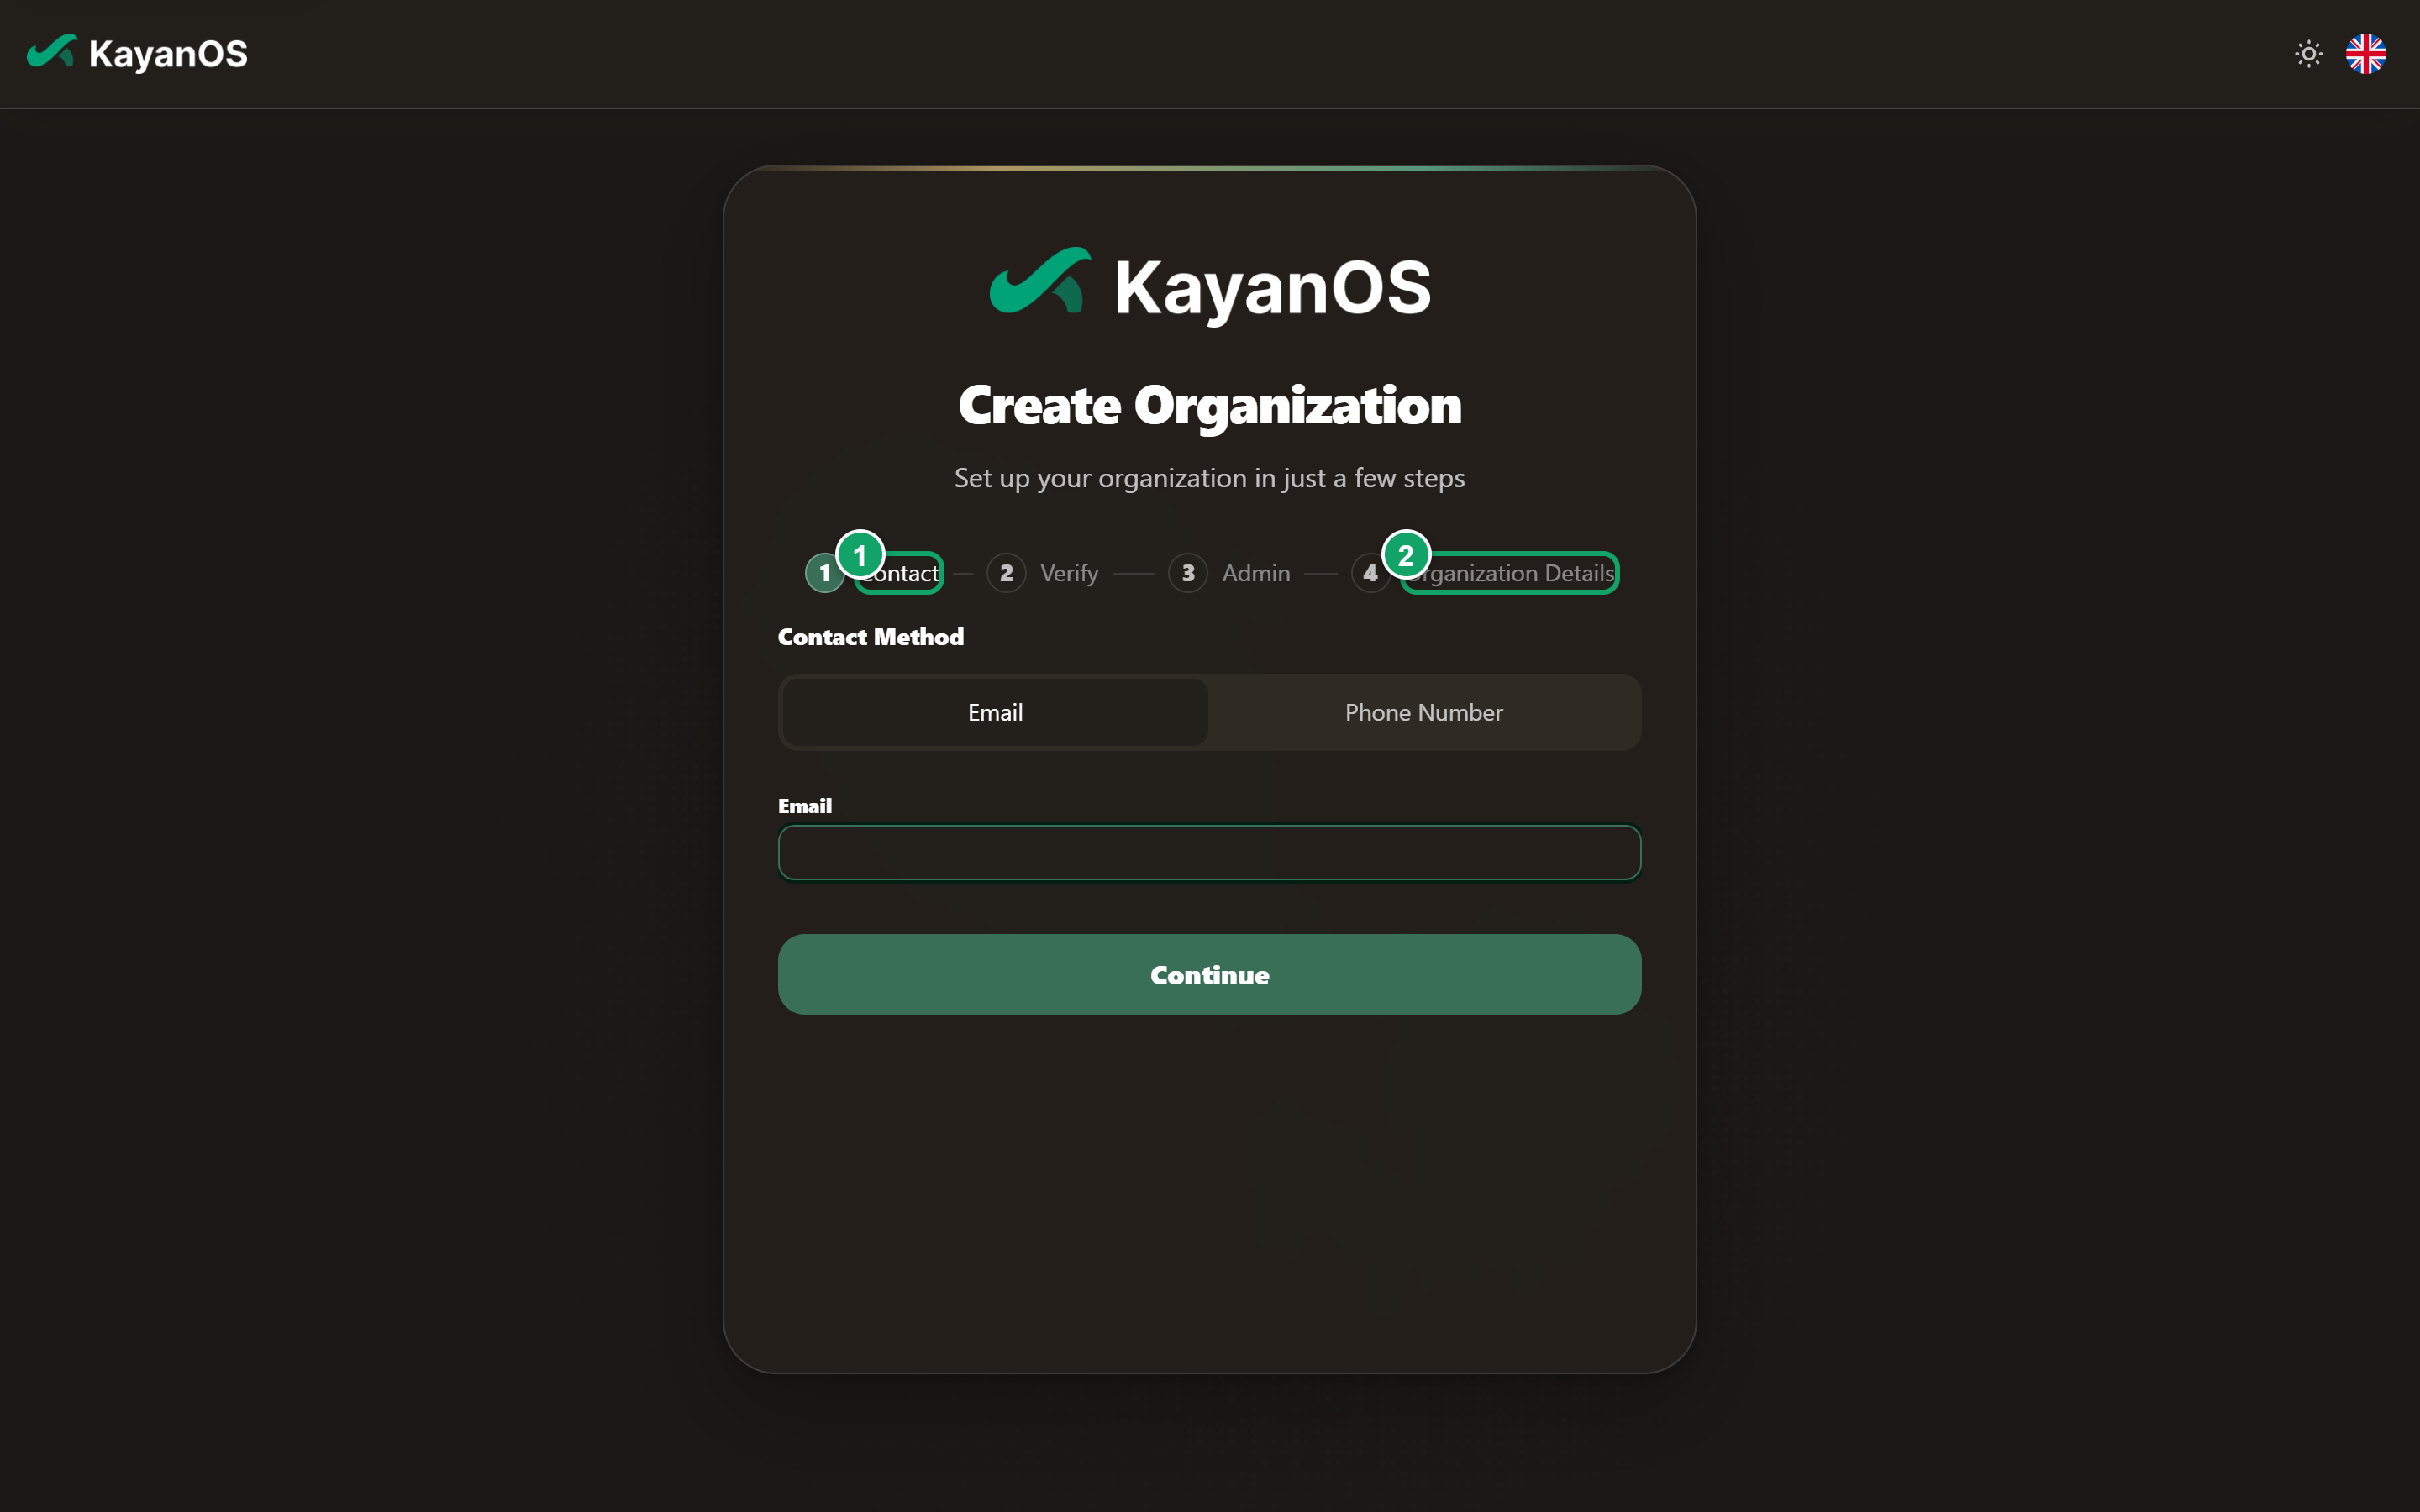
\includegraphics[width=0.95\linewidth,height=0.72\textheight,keepaspectratio]{figures/screens/ch02-create-org-en.png}
\caption{The “Create Organization” page and its four steps}
\label{fig:setup-create-screen}
\shotnote{The “Create Organization” page splits the process into four consecutive steps, from “Contact” to “Organization Details”; the highlighted number marks the current step. The current step’s fields appear under the step bar, and the other steps follow in the order described in the list below. Numbers on the image: ① The first step, contact details, where you start. ② The last step, organization details, where you finish.}
\end{figure}

\begin{enumerate}
  \item Contact: enter email or phone.
  \item Verify: enter the 6-digit code within 10 minutes. Request another after one minute.
  \item Admin: enter your name and an optional password.
  \item Organization Details: enter subdomain, name, country and staff range; optionally add a logo. Complete creation.
\end{enumerate}

\textbf{Check:} sign in at the new address as administrator and confirm the organization name. Keep the address for the team.

\begin{rcnote}[Subdomain]
Use 3–63 lowercase letters, digits or hyphens. No leading/trailing hyphen, existing address or reserved name such as admin.
\end{rcnote}

\begin{table}[H]
\centering
\caption{What you find ready and what you need to enter}
\label{tab:setup-generated}
\rcZebra
\begin{tabularx}{\linewidth}{Y Y}
\rcHeaderRow
\thh{Ready after creation} & \thh{Add later in HR}\\
Your account as a member, with the “Administrator” role. & Locations (places of work).\\
The basic roles. & Nodes (organizational units).\\
The apps and entity definitions. & Positions.\\
Currencies and status templates. & Members, assignments and shifts.\\
\end{tabularx}
\end{table}

\section{2. Organization settings}
\label{sec:setup-settings}

\textbf{Open:} Settings / Management / Organization settings. Review the following settings right after creating the organization, because their defaults may not suit your work.

\begin{table}[H]
\centering
\caption{Settings to review right away}
\label{tab:setup-settings}
\rcZebra
\begin{tabularx}{\linewidth}{R{4.2cm} R{2.6cm} Y}
\rcHeaderRow
\thh{Setting} & \thh{Default value} & \thh{Why does it matter?}\\
Default timezone & UTC & Sets the times of working hours, appointments and reports.\\
Default language & English & The interface language for new members.\\
Start day of week & Monday & Affects the calendar and weekly reports.\\
Logo and primary color & — & The organization's identity in the interface (optional).\\
\end{tabularx}
\end{table}

Choose the time zone, language and start of the working week. Save and reopen to check.

\begin{rcnote}[Example: Horizon]
Horizon chooses the Asia/Damascus time zone and Arabic; it sets the start of week to the day the organization has agreed on.
\end{rcnote}

\section{Check the result}
\label{sec:setup-check}

\begin{rcchecklist}[Checklist: setup complete]
\begin{checklist}
  \item You can sign in at the organization address as administrator and see the correct organization name.
  \item The time zone, default language and start of week remain correct when you reopen settings.
  \item You have kept the sign-in address for use when adding the team later.
\end{checklist}
\end{rcchecklist}

\section{Problems and fixes}
\label{sec:setup-errors}

\begin{table}[H]
\centering
\caption{Problems and fixes}
\label{tab:setup-errors}
\rcZebra
\begin{tabularx}{\linewidth}{R{4.2cm} Y Y}
\rcHeaderRow
\thh{The problem} & \thh{The cause} & \thh{The fix}\\
Subdomain rejected & In use, reserved, or contains characters that are not allowed. & Choose another name with lowercase letters and numbers.\\
Verification code expired & 10 minutes have passed. & Ask for a new code.\\
Wrong times & The timezone is still UTC. & Change it in Organization settings.\\
\end{tabularx}
\end{table}

\section{Continue with team setup}
\label{sec:setup-next}

The organization is ready for work records. Continue to Chapter~\ref{ch:hr} to set up the team; it explains the pages, fields and practical examples.

\begin{itemize}
  \item For departments and work sites: Nodes in Section~\ref{sec:hr-feature-nodes} and Locations in Section~\ref{sec:hr-feature-locations}.
  \item To add employees and jobs and link them: Members in Section~\ref{sec:hr-feature-members}, Positions in Section~\ref{sec:hr-feature-positions} and Assignments in Section~\ref{sec:hr-feature-assignments}.
\end{itemize}

\begin{rcnote}[Example: Horizon]
After the organization settings are saved, Sarah starts setting up departments, locations and employee records using the HR pages. She then continues with attendance, leave and payroll as the organization needs them.
\end{rcnote}
